\subsection{Synchronized Console}

For consistency inside outputs, we needed to implement synchronization
mechanisms. To do that, we choose to use the \textbf{Monitor} concurrent
programming model.\\
Each methods of the synchconsole was encapsulated using two
semaphores :
\begin{itemize}
    \item one for read \textbf{read} (GetInt, GetString, GetChar)
    \item one for \textbf{write} (PutInt, PutString, PutChar).
\end{itemize}

As GetString/GetInt and PutString/PutInt call respectively GetChar and PutChar,
we either need recursive semaphores or make internals sub-routines
\_GetChar/\_PutChar which are called by GetString/GetInt/GetChar, letting the
synchronization mechanism inside these calling methods.\\
The second choice was made for simplicity.\\

To conclude with synchronized console implementation choices, we had to handle
error inside GetChar and GetInt :
\begin{itemize}
    \item For GetChar, the choice was made to return an integer instead of a char. By
convention, \textbf{EOF} is $-1$.
    \item For GetInt, we cannot used a long int because the return value of a syscall is
inside a register which is of size $4$. Thus the address of an int is needed by
GetInt. This int will be filled with the getting number and the return value of
GetInt is used to handle error (see user documentation for more information).
\end{itemize}

\subsection{Multi-Threads}

Concerning stacks management, the first kernel thread (created at \emph{Nachos}
start) use the UNIX-process stack. Other kernel threads use heap-allocated
stacks. For user thread, each thread as his own stack, from bottom of the memory
up to the top. All user thread stacks are handled inside StackMgr class.
StackMgr handle all stacks requests inside a AddrSpace. If UserThreadCreate is
called and no space for stack is available, the function returns $-1$.\\

A word about thread hierarchy. There is none. This mean that every thread
belongs to a process. A thread can create other threads but the behavior (e.g
exit) does not influence others.

A user thread can exit in two ways :
\begin{itemize}
    \item calling \textrm{UserThreadExit(void *ret)} where $ret$ is a generic
        pointer to the returned data
    \item returning from the thread function (also a generic pointer)
\end{itemize}

%One exception is for the first thread (the one with the main function). As
There is an exception for the first thread (the one with the main function). As
pthread implementation, calling \textrm{UserThreadExit} with main thread let
other threads finish. After the last thread end, it will exit the process.\\

As threads are light-weight processes, calling \textrm{Exit} in any threads
kill the process with all threads belonging to it. This is the same if the main
thread reach the return of the main function. It will implicitly call
\textrm{Exit}. Thus does not wait for threads termination.\\

It is noticeable that thread id (tid) are unique to a process during is
lifetime. A tid will never be re-used. This allows us to implement
\textrm{UserThreadJoin} as discussed below. Even after a thread termination, his
AddrSpace keeps track of its statue and keep a Semaphore to join on it as well
as the pthread return value if available.

\textrm{UserThreadJoin(unsigned int tid, void **retval)} allows one thread to wait for
another.\\
Inside retval (if not NULL) you can get the value return either by
\textrm{UserThreadExit} or by the return value of thread function. If that
thread has already terminated, then \textrm{UserThreadExit} returns
immediately.\\
If multiple threads simultaneously try to join with the same thread, only the
first one will be able to join on it. For others, syscall will return error
code $-2$. \\
If threads join multiple times on the same thread (not at the same time), each
call will be successful and if retval is not NULL, it will be filled with the
return value of thread.\\

About semaphores, they are now available to user program using
UserSemaphoreCreate syscall. This return a semaphore id process-specific. To
wait for resource being available, \textrm{UserSemaphoreP} is here. To notify resource
availability, it's\textrm{ UserSemaphoreV}. Finally,\textrm{ UserSemaphoreDestroy} destroys a
semaphore. Semaphore id are process-unique and not re-used. If a
UserSemaphore[P|V] is used after the semaphore was destroyed, these syscalls
will return $-1$. All semaphores are destroyed at the end of a process.

\subsection{Virtual Memory}

To handle virtual memory, all requests for memory page allocation/deallocation
was made through a FrameProvider. This component has his own frame placement
policy. Everytime a process (via his AddrSpace) ask the FrameProvider for
physical pages when it is needed (for Stack, Heap or Code/Data segments).
We implemented different strategies to see if our model was coherent : random,
first and last.\\

A heap management was implemented. Stack and heap have fixed max size and
we let a page between both in order to throw a page fault we try to access
outside the bounds. A HeapMgr which embed a top heap pointer manage requests for
new heap pages.
Heap and stack pages are dynamically allocated using FrameProvider.

\subsection{Multi-Processes}
ForkExec creates new kernel thread that will execute new user program in a new
address space. The creation of the new process is divided between the calling
thread and the called thread which will begin its execution with a special
initialization function. The managing of the processes is done by the processMgr
object which manages the pids and the ability to wait for a certain thread using
Waitpid function.\\

There is no processes hierarchy, only the number of currently running threads is
counted and when the last process exit the machine is halted.

When a process halt it does not affect the others since all are independent
programs with their own virtual memory code, data, and stacks.\\

Each pid is unique so when using Waitpid it is possible to know and prevent the
process from waiting on a dead process or on itself. And as such it is possible
to avoid deadlocks that would happen otherwise.

Waitpid allows to catch the exit code of the process which is being waited.

\subsection{FileSystem}
For Filesystem, we followed the subject.

\subsubsection{Sub-Directory and Current Directory}

We added an attribute inside the directory table. This attribute ($isDir$) allows
to distinguish between files and directory. A function called
\textrm{ExpandFilename} handle all ``.'', ``..'' to compute the absolute
path. This allows us to avoid creating two special files inside each directory,
saving two entries.\\

A notion of CurrentDirectory was implemented attached to a process. Each process
has his own directory and relative path are computed taking into account this
one. All paths are computed using ExpandFilename.

\subsubsection{Open file table}
Each process has his own file table which is typically a unique identifier and a
FileInfo structure. This file structure allows checking which thread own the
file, which file name was already opened to apply some restrictions.

\subsubsection{Max File Size and Dynamic Size}
By default, each file was limited to $\frac{SectorSize - 2*4)}{4} * SectorSize$
bytes ($3.75K$). Either the $SectorSize$ needs to be extended, or another
indirection level was added.
Now the $\frac{SectorSize - 2*4}{4}$ data sectors of a FileHdr points to
DataBlockHdr. Each of these DataBlockHdr points to $\frac{SectorSize}{4}$ data
block (the real content).
The maximum size is now of $(\frac{SectorSize - 2*4}{4} +
\frac{SectorSize}{4})*SectorSize$ bytes ($122kB$).\\

When a file is created, it has a size of $0$. At each write, if needed, file size is
expanded allocating Data Sector and DataBlock sector.

\subsubsection{Concurrent Accesses}
The SynchFileMgr component manages all concurrent accesses to a same file
(represented by the sector of his FileHdr). Attached to this sector, a
ReaderLock and a WriterLock are used for implementing a reader/writer schema for
all file accesses across all processes and threads.

\subsection{Network}
We chose to implement a socket user interface in our Nachos kernel. These
sockets work in connected mode with robust transmissions.\\
As in TCP sockets, a server create a listening socket and accept new
connections on it. This allow to join a server on one port (defined by
convention as $80$ for HTTP servers) with many clients, and each of them will then
have a personal socket with the server.
On its side, the server can communicate with each client separately on
different sockets. Our kernel provides $16$ ports which can handle $16$ sockets
each, so the kernel can handle $256$ connections at a time.

\subsection{Low level transmission}
The lower layer of our network implementation is the transmission of one mail.
This part have to be robust and then we can construct an higher level protocol
on it.\\
For every single mail, the emitter send the mail, wait a confirmation and retry
if no. The number of tries is limited and the send function will return an
error if this limit is reached.
The receiver can receive many times the same mail before the emitter receive a
confirmation. To prevent the duplication of a mail, we include an id in each of
them. The receiver will take the first iteration of a mail and just confirm the
other. The id we use is an int which is always incremented, so the socket will stop
to work after $2^{32}$ mails sent. This limit is hard to reach, so we did not
deal with it, but it is possible to make the id go back to $0$ when it happens
without blocking the network.
A confirmation mail contains the id of the mail it confirm, so a confirmation
mail cannot be used later by the emitter to confirm an other mail.

\subsection{Protocol}
Then we constructed the connected protocol over the robust transmission.
The connection establishing use a three-way handshake.\\
We use the mailboxes of the initial Nachos code as ports, but now each mailbox contains an array of 
socket because many sockets can be connected within a same port (for instance the
port $80$ of HTTP servers).  The number of connections a port can handle is limited 
to $16$, because an array was simpler to implement and $16$ is sufficient (but it 
can be replaced easily by a list).\\
The postal worker dispatch the mails he receive. He know in which mailbox
thanks to the mail header and then find the good socket by comparing the origin
of the mail to the ones contained into sockets.\\
Here is the schema of the classes used in network :
\begin{figure}[H]
	\centering
		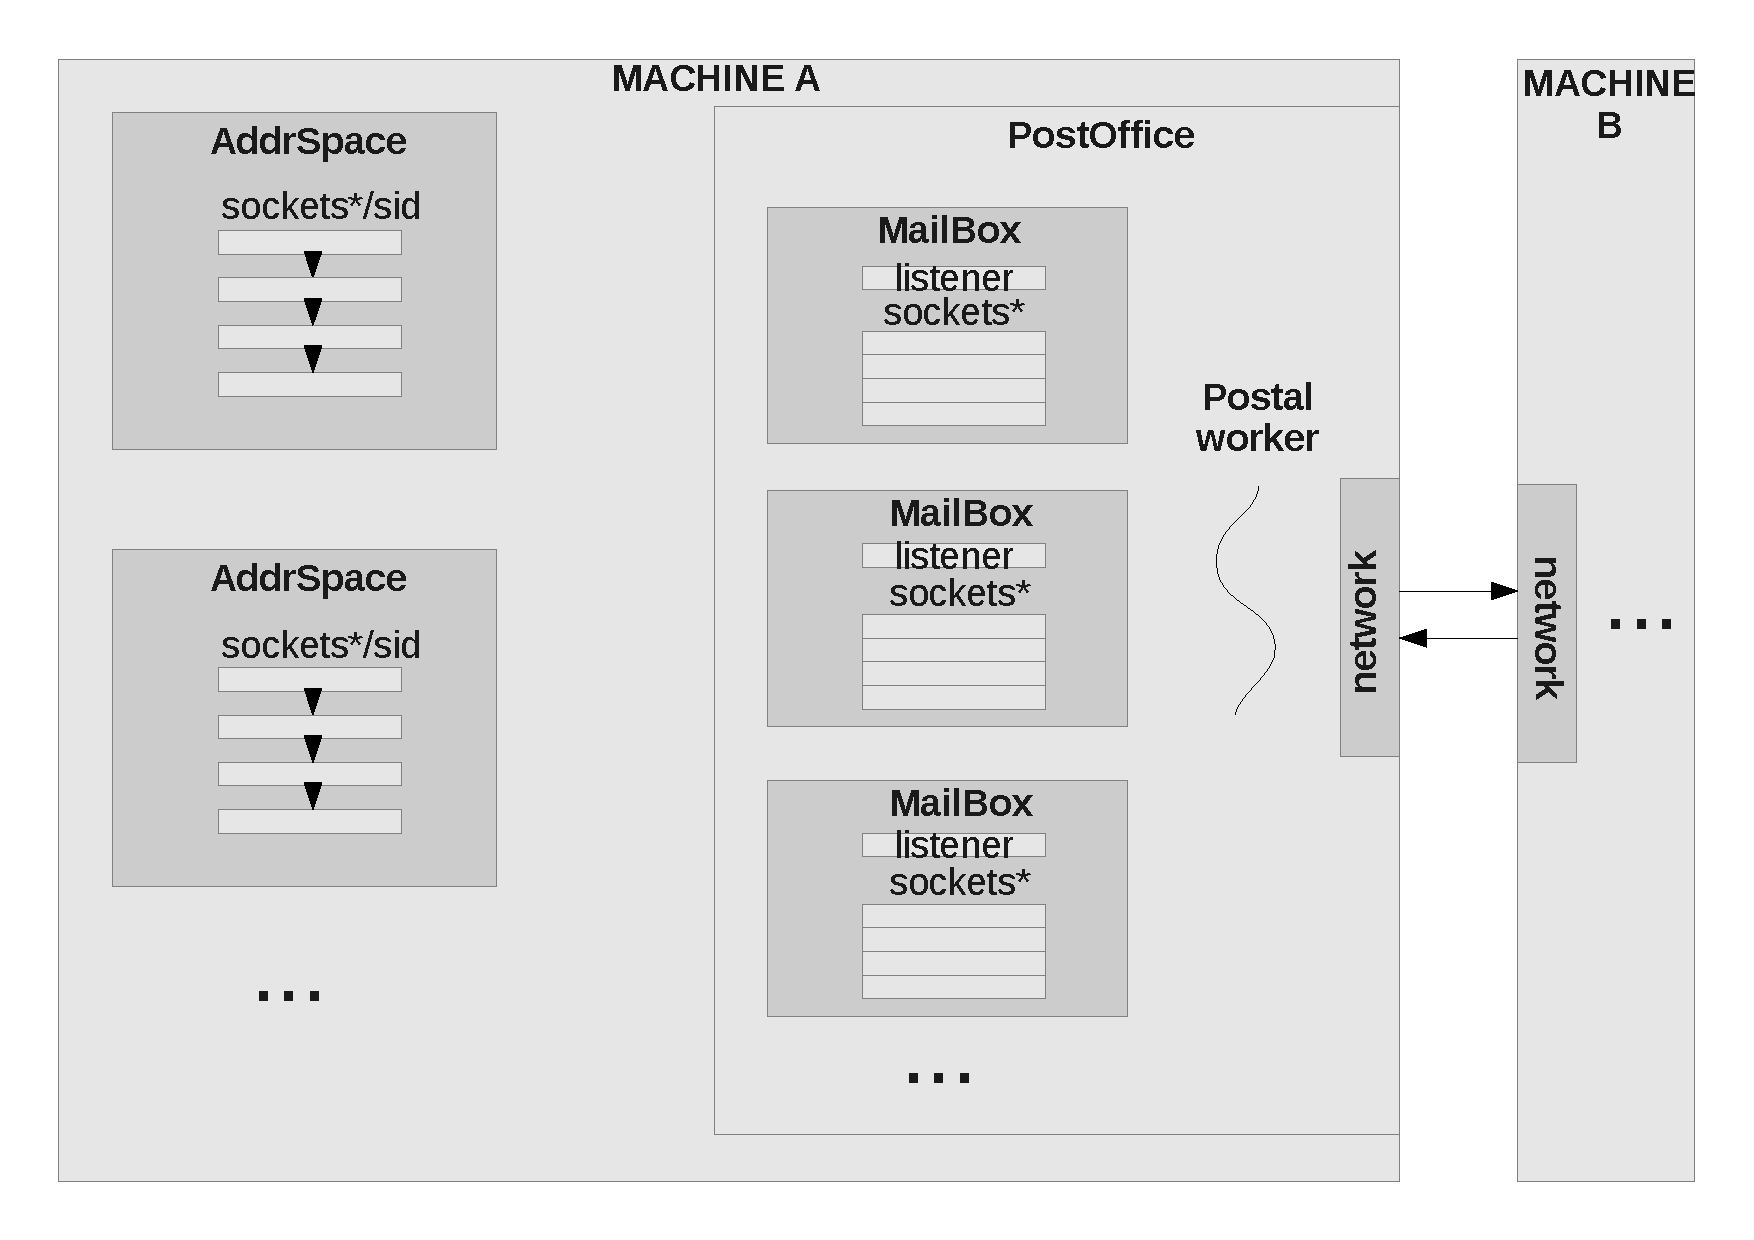
\includegraphics[scale=0.4]{networkschema}
		\caption{Each socket can be accessed from its address space and the mailbox which handle it.}
\end{figure}
%%% Local Variables:
%%% mode: latex
%%% TeX-master: "report_nachos"
%%% End:
